\documentclass[12pt]{article}
%Required: You must have these
\usepackage{graphicx}
\usepackage{tabularx}
\usepackage{natbib}

\usepackage{array}
\usepackage{amsmath}
%\usepackage[backend=bibtex]{biblatex}
\setkeys{Gin}{width=0.8\textwidth}
%\setlength{\captionmargin}{30pt}
\setlength{\abovecaptionskip}{10pt}
\setlength{\belowcaptionskip}{10pt}
 \topmargin -1.5cm 
 \oddsidemargin -0.04cm 
 \evensidemargin -0.04cm 
 \textwidth 16.59cm
 \textheight 21.94cm 
 \parskip 7.2pt 
\renewcommand{\baselinestretch}{1.2} 	
\parindent 0pt


\bibliographystyle{..//refs/styles/besjournals.bst}
%\usepackage{xr-hyper}
\usepackage{hyperref}
\title{Thermoperiodicity}
\begin{document}
\begin{enumerate}
Note could define: Full factorial, orthoginal, periodicity, intesity, forcing as a box maybe to shorten main text?\\

\section{Introduction}
\item Temperature and light control and signal many biological processes.
\item They often interact, substitute or compensate for each other.
\item A major goal of biology is to quantify their effects and interactions
\item This has become extra important for predicting organism's response to global change
\item This task cannot be done well through observational studies as light and temperature regimes usually covary
\item Experiments in controlled environments (growth chambers, greenhouses etc) can do this, using experimental treatment to partition the effects of this variables and their interactions.
\item Indeed much progress has been made with this apporach
\item But experiments must balance many competing factors in their designs, biological realism with statistical interence, the effect of unmeasure climate variable, blocking effects etc.
\item In the sections below we highlight a particular problem that can arise when designing experiments to partition the effects of temperature and daylength and understand their interaction. Our example uses woody plant phenology as an example, but the approach we detail here is relevant for other organisms and biological process too.
\end{enumerate}

\section{Phenological response to Temperature and Light}
Here a very brief (one paragraph) overview of how light and temperature influence spring phenology. Keep it basic (Warming accelerate phenology, photoperiod might be a threshhold), aknoledge chilling is important too, but our example won't really focus on it. Leave some open questions about their interactive nature

\section{Testing Interactions}
\begin{enumerate}
\item To test interactions and partition effects amoung two variables that covary in nature one must:
\item Have at least 2 treatment levels of each variable of interest
\item Apply them orthoganigally, factorially (\ref{fig:examp}, blue box) and define these terms.
\item This may seem obvious but is rarely done. In the case of phenology, a recent analysis of controlled enviroonment study found that only X of Y studies manipulated both light and temperature cues in the same experience and only Z of X did so orthoginally.
\end{enumerate}
\section{Axes of environmental variation annd their there problem}
\begin{enumerate}
\item A further complication arises when decided how to apply each treatment.
\item For any environmental variable there are two axes of variation that can be manipulated in an experiment.  
\item Intensity: Temperature, luminocity. 
\item Period: Thermoperid, Photoperiod.
\item There are measures that incorperate both period intensity (ie growing degree hours).
\item For light cues, photoperiod is the primary phenolgoical cure
\item For temperature, period and intesity matter. For example, temperture in nature varies diurnally and dirunal temperature fluctions may contribute to the phenology signal, or at the very least, lack of them might make phenology wonky. 
\item Therefore a common approach in experiments that seems to balance prior knowlege, biological realism and experimental inferences is to vary photo period, and temperature intensity and period. 
\item Clarify with an example. 12 and 8 hours of daylength. 30/20 and  20/10 temperature (or whatever I said in the figure).
\item If not carefully handled this approach can introduce a nonorthogicanity into the experiment, biasing inference.
\item If the thermo-periodicity and photoperiodcity are coupled (ie the night time temperatures begin when the lights go off, and the day time temperatures begin when they turn back on) The impact is that that the high temperautre high/long photoperod treatment more cumulative heat than the high temperature/short photoperiod treatment throughout the experiment as can be seem when the temperature treatment are converted to thermal sums (\ref{fig:examp},(\ref{fig:ortho}b)). To state this more simply, though the applied temperatures are the same sicne their are applied for different durations, the mean daily temperature differ among the temperature treatments.
\item This non-orthoginality makes it stasticially impossible to differentiate the effect of the photoperiod and temperature treatments.
\end{enumerate}
\section{Quantifying uncertainty}
\begin{enumerate}
\item To estimate the extent to which this non-orthangonical could bias results we intergated the results from a large scale experiment that included a coupled thermo-photoperid design. We used plane geometry to estimate how much of the estimated forcing effect (the assumed dominant cue) may actually be attributed to change in photoperiod. The calcualtions can be found in the suppliment.
\item While the original model estimates of the forcing and photoperiod effects (phenological sensitivy; $\Delta$ phenological event day/ $\Delta$ cue level) were estimate 9.5 and 4.5 advance we estimate that as much about 3.0 (units?) of the forcing effect could be attributed to the photoperiod effect.
\item It is important to stress that this is not a model correction. The original model could acutally before correct or it could in fact have understimated the true forcing effect and infalted the photoperiod effect. We simply cannot say this. (\textit{Probably should think about how to phase all this without making it seem like the Flynn paper is wrong}).
\item Our estimate of ``how much of the reported photo-period response could in actuality be driven by the latent differences in thermo-period" can be rephrased as a prediction of the expected difference in estimated photoperiod sensitivity between a coupled and decoupled photo- and thermo-period experiment.
\item While we are aware of no experiments that explicitly test these different designs, a phenological study by \citet{Buonaiuto2020} applied serveral treatments levels that overlap with those in the \citet{Flynn2018} study to twig cuttings from the same source population. However in the second study the authors decoupled photo- and thermo-period. After subseting each dataset to  include nly species and treatment levels common amoung them, we re-analyzed the data (see supplimental method) and found that difference in the average response to photoperiod amoung study designs  was on the same order our mathmatical prediction see figure, though the photoperiod effect was in fact weaker in the uncoupled dataset (\ref{tab:compy}).\\
\item  With such significant uncertainty in partitioning the effect of forcing and photoperod even in experiment, this might contribute to the debate about the importance of photoperiod.
\item Below we outline several solutions to this experimental design, that should inprove the inference from growth chamber studies
\end{enumerate}

\section{Solutions}
\begin{enumerate}
\item Manipulate temperature intesity only and photoperiod. You estimate interactions because you have multiple levels of temperature and orthogiality. Lose some biological realism (\ref{fig:ortho}a).


\item Uncouple thermoperiod and photoperiod. As done in \citet{Buonaiuto2020}. While this is probably better than coupled approach as it account for statistical interaction, it may introduce new artifact that occur from biological interactions. For example evidence from horticulture studies have demonstrated that cell growth is most sensitive to temperature fluctuation at the beginning of the photoperiod\citep{Erwin1998}. \citet{Erwin1998} found that increasing temperatures in the first two hours of the photoperiod was almost as effective for stimulating shoot elongation as similar temperature increases for the whole photoperiod (\ref{fig:ortho}c).

\item Set temperature treatments using metrics that account for period and intestist. Growing degree hours.maintain mean temperature and set photoperiod legnths and thus thermal orthoginality in expiriment by proportionately varying diurnal fluctionation accross treatment level. However, if the differenes between day and night temperature has a meanful biological effect as has been shown, this introduces another confonding, non-orthoginal factor (\ref{fig:ortho}d).

\item While this improvements should improve our ability to assess light and temperature interactions in biology, their challenges should aslo remind us to be humble with inference and think critically about what is, and isn't accounted for.
\end{enumerate}



\begin{table}[h!]
    \centering
\begin{tabular}{|c|c|c|}
\hline
& predicted difference & observed difference (sd)\\
\hline
budburst sensitivty & 3.0 & -4.1575777(2.665567)\\
\hline

\end{tabular}
 \caption{Need a caption, and maybe a better way to show this, and to recheck the analyses}
     \label{tab:compy}
\end{table}

\begin{figure}[h!]
    \centering
 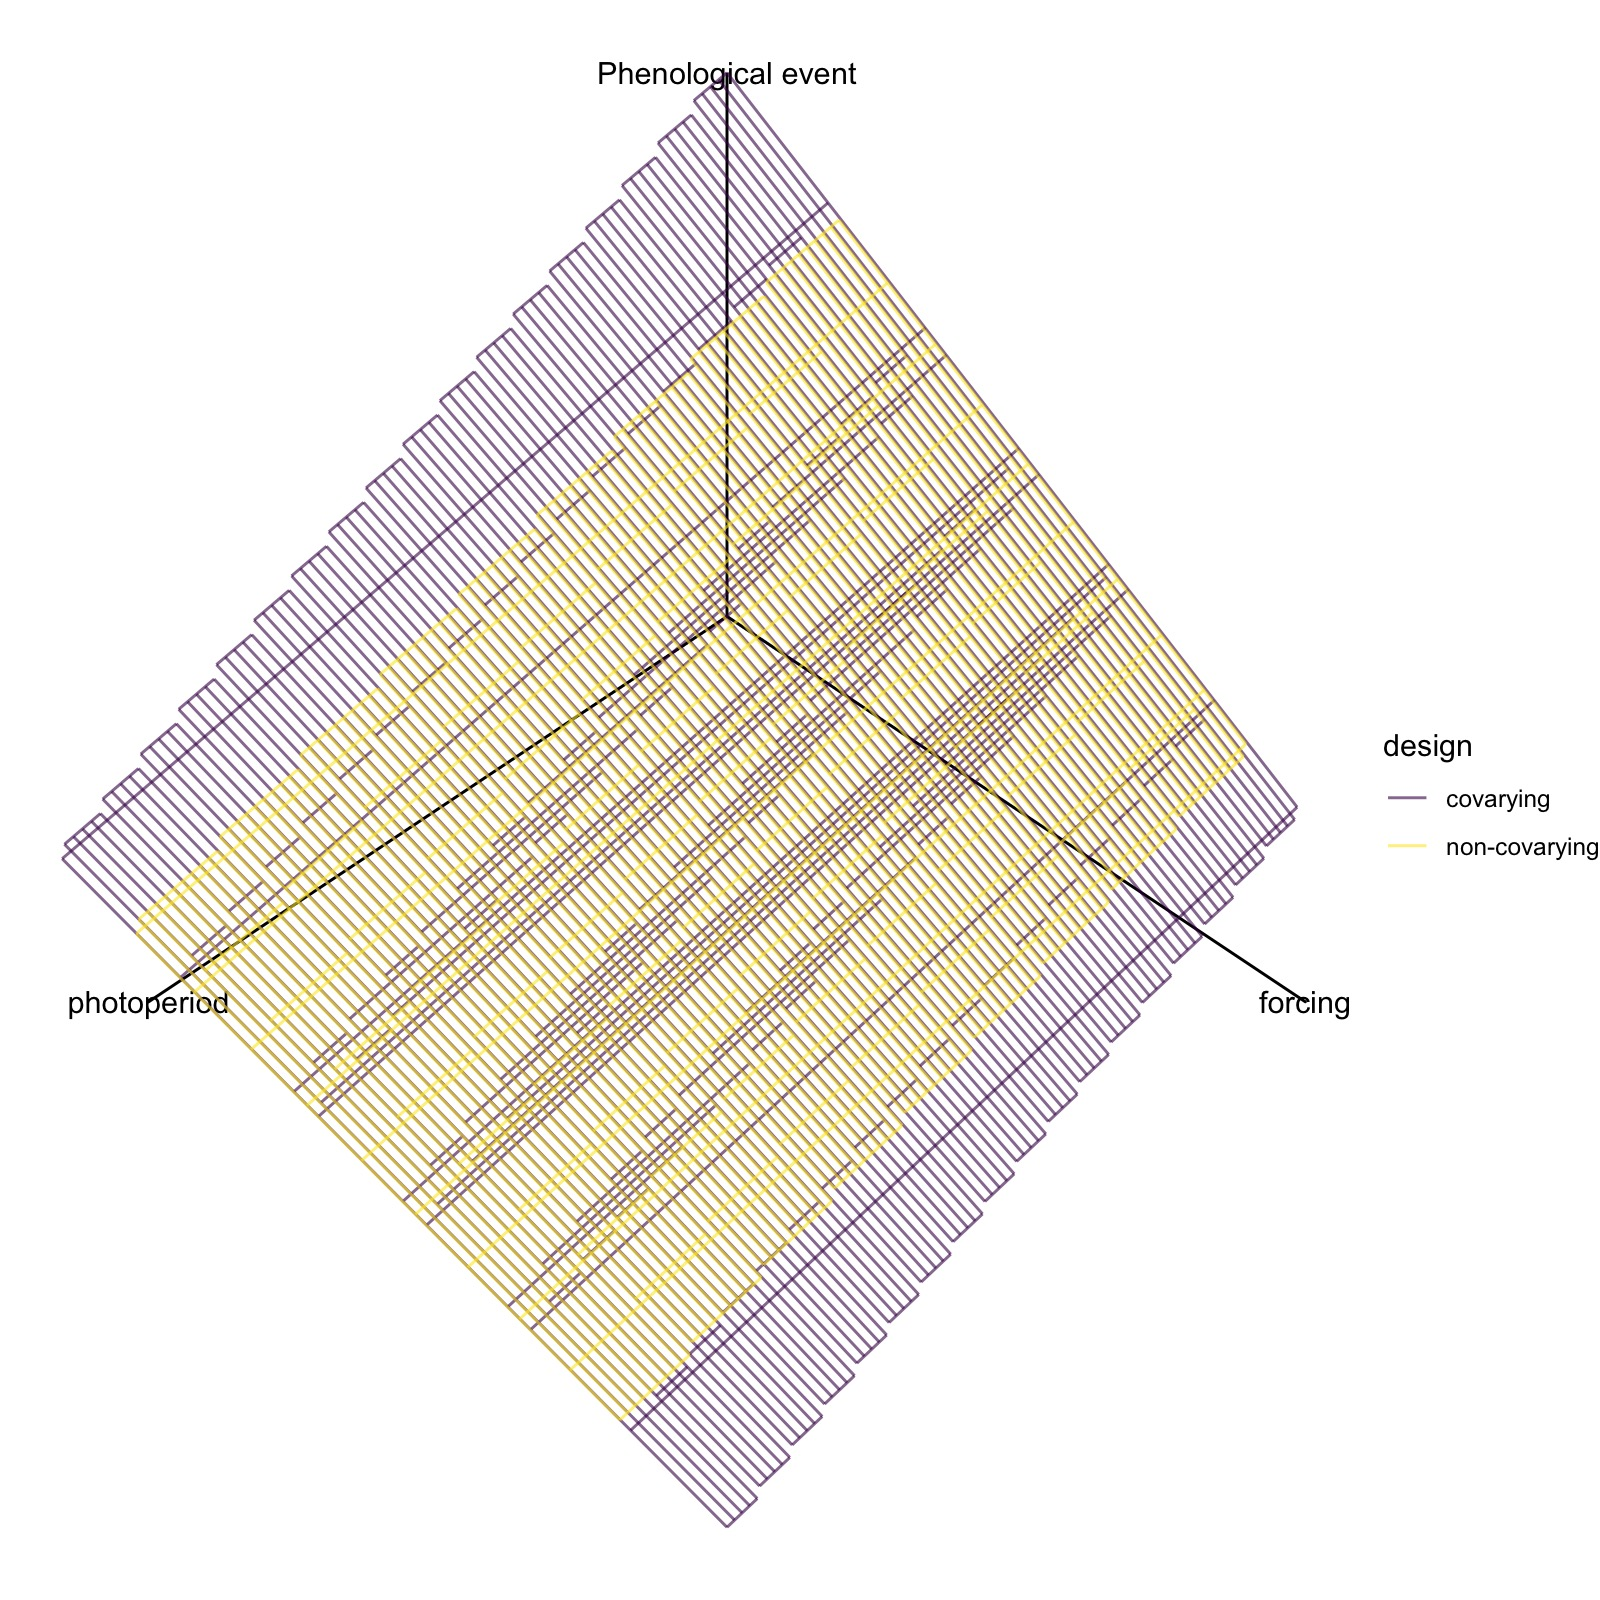
\includegraphics[width=\textwidth]{..//Plots/periodicity_figures/orthog.jpeg}
    \caption{To partition the effects of light and temperature and their interactions in experiments,  treatments must  must apply at least two treatment levels of each variable and be full factorialAand orthoginal, that is all possible combination of treatments levels applied and each is independent of the other (blue rectagle). When a daily thermoperiod and photoperiods are coupled, a latent non-orthognality is introduce as the long photoperiod/ high temperature treatment combination will recieve more daily heat exposure (thermal sums) than the short photoperiod/high temperautre combination despite having the same temperature settings. }
    \label{fig:examp}
\end{figure}

\begin{figure}[h!]
    \centering
 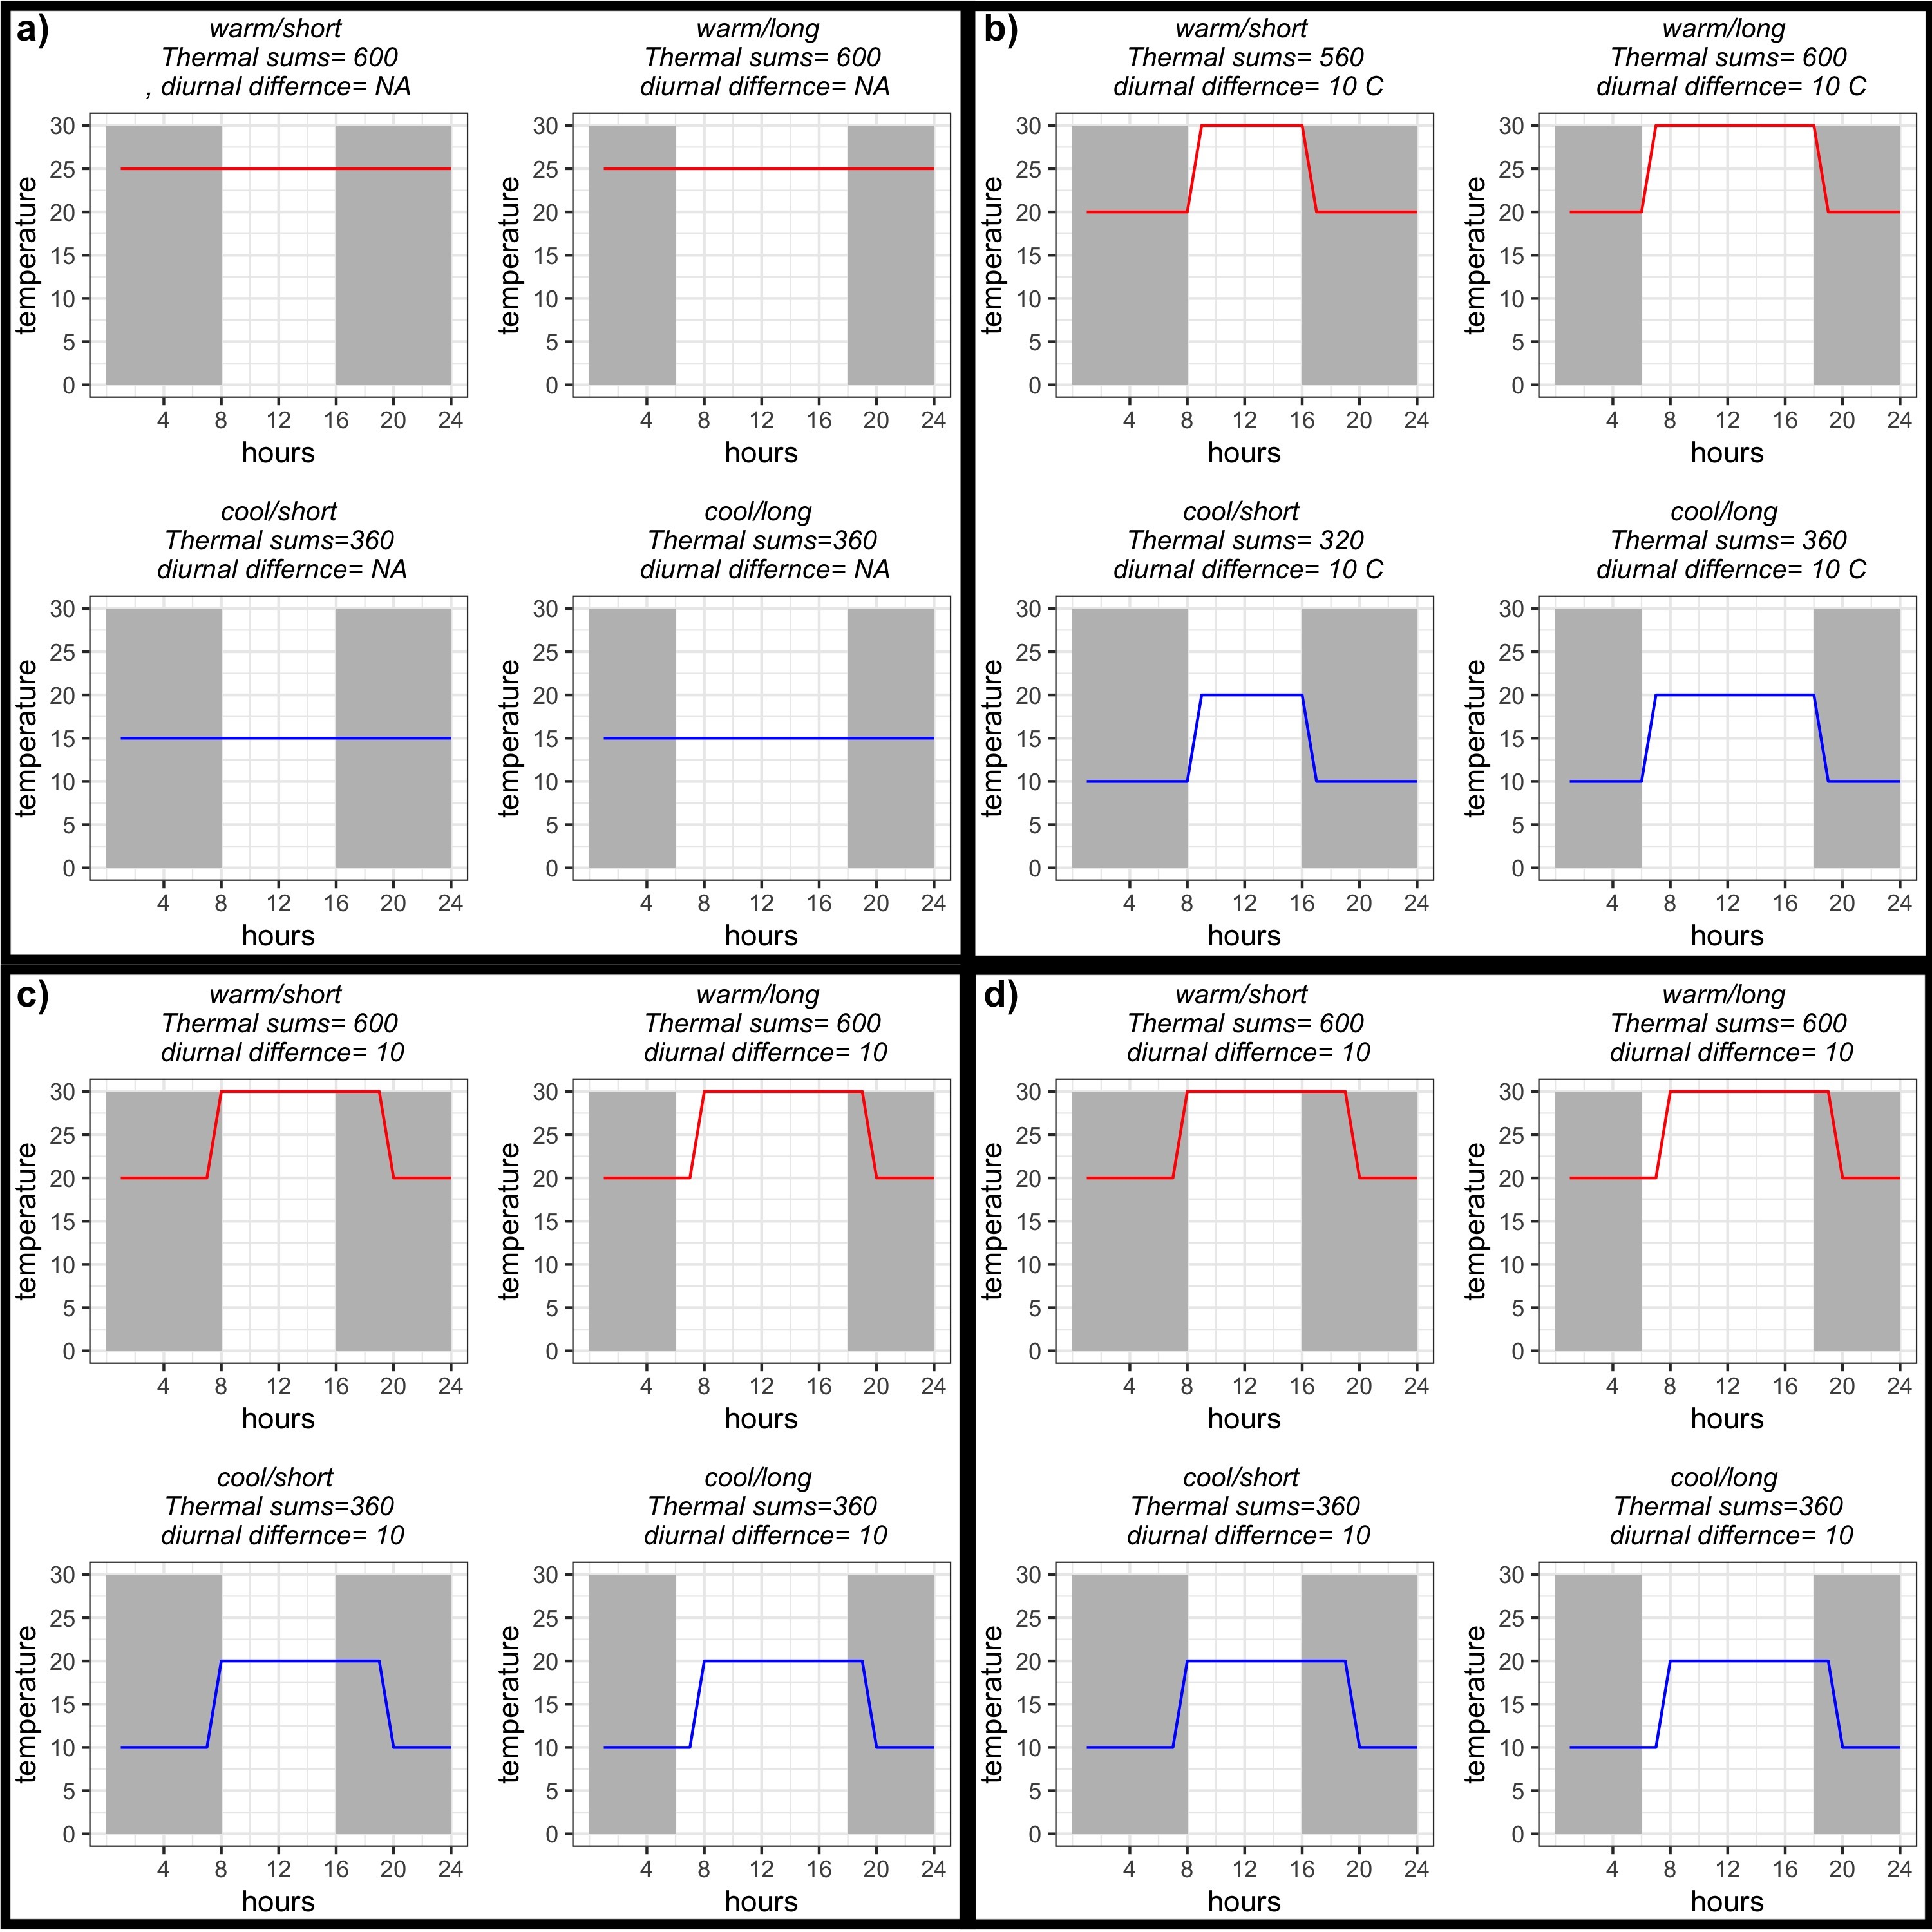
\includegraphics[width=\textwidth]{..//Plots/periodicity_figures/designs.jpeg}
    \caption{Conceptualized experimental designs to test temperature and daylength interactions on a biological response. All four designs apply two treatment levels of forcing temperatures and two treatment levels of photoperiod yet differences how the thermoperiods are varied relative to photoperiod in each scenario impact the orthoginality of the treatment spacies, compromsing its inference. Design \textbf{a)} is orthoginal in temperature and photoperiod, but lack thermoperiod, sacraficing biological realism and comprimising any responses that require durnal temperature fluctions. Design \textbf{b)} incorperates a standardize diurnal temperature fluctuation across all treatment, but because this thermoperiod is coupled with the photoperiod, the daily thermal sums across treatments are non-orthoginal. In \textbf{c)} the standard diurnal temperature fluctuation is maintained but thermoperiod and photoperiod are decoupled and varied independently, maintaining orthoginality in heat sums across treatment combinations. In design \textbf{d)} photo and thermo periods are coupled and orthoginality are maintained by proportionately varying the diurnal temperature fluctations across treatments, introducing a new latent difference among the treatments.}
    \label{fig:ortho}
\end{figure}
 
 

\end{document}